\documentclass[11pt,a4paper]{article}

\usepackage[utf8]{inputenc}
\usepackage[T1]{fontenc}
\usepackage[french]{babel}
\usepackage{lmodern}
\usepackage[margin=2.4cm]{geometry}
\usepackage{graphicx}
\usepackage{amsmath,amssymb}
\usepackage{booktabs}
\usepackage{caption}
\usepackage{subcaption}
\usepackage{float}
\usepackage{xcolor}
\usepackage[colorlinks=true,linkcolor=blue!60!black,urlcolor=blue!60!black]{hyperref}

\graphicspath{{figs/}}
\captionsetup{font=small,labelfont=bf}
\setlength{\parskip}{0.4em}
\setlength{\parindent}{0pt}

\newcommand{\alert}[1]{\textcolor{red!70!black}{\textbf{#1}}}

\title{\textbf{Absentéisme au travail}\\[0.3em]
\large Analyse de séries temporelles \& classification}
\author{Berthelot Samuel \and Maeva Ange Koumo}

\begin{document}
\maketitle

\begin{abstract}
      \noindent
      On étudie un jeu de \textbf{740 absences} enregistrées chez un transporteur brésilien
      entre juillet 2007 et juillet 2010. Deux questions guident le travail :
      \begin{itemize}
            \item[(i)] peut-on \textbf{prévoir} le volume mensuel d'heures d'absence~;
            \item[(ii)] peut-on \textbf{expliquer / classer} la durée d'une absence à partir
                  de ses caractéristiques~?
      \end{itemize}
      L'analyse de séries temporelles montre une série \emph{proche d'un bruit blanc}
      (prévision peu utile), ce qui motive un pivot vers une \textbf{approche explicative} :
      effet du jour de la semaine puis classification de la durée en trois classes.
\end{abstract}

\newpage
\tableofcontents
\newpage

%======================================================
\section{Contexte \& données}

Le jeu de données (UCI \#445) recense des absences individuelles décrites par 20 variables
(motif codé CIM/ICD, jour de la semaine, saison, distance domicile--travail, charge de
travail, IMC, etc.) et la cible \texttt{Absenteeism time in hours}.

\textbf{Reconstruction temporelle.} Il n'existe pas de colonne de date : les enregistrements
sont seulement ordonnés chronologiquement. On reconstruit un index mensuel à partir de la
variable \texttt{Month of absence} (en incrémentant l'année à chaque retour en arrière du
mois), puis on agrège le \textbf{total d'heures par mois}. On obtient une série mensuelle de
\textbf{37 points} (figure~\ref{fig:serie}).

\begin{figure}[H]
      \centering
      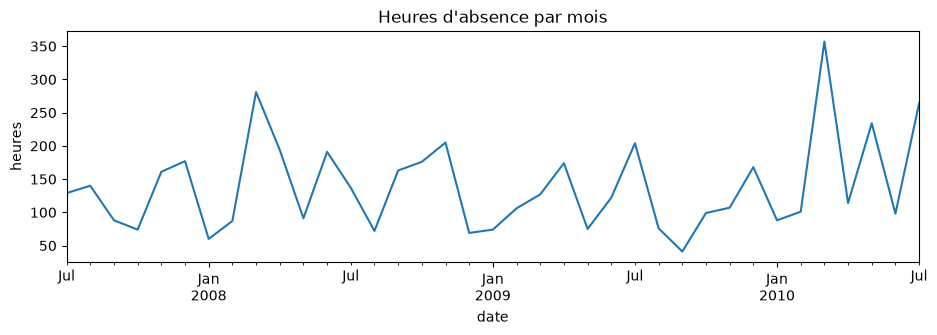
\includegraphics[width=0.82\linewidth]{serie}
      \caption{Heures d'absence par mois (juil.~2007 → juil.~2010). Série courte et bruitée, avec un pic marqué début 2010.}
      \label{fig:serie}
\end{figure}

Deux problématiques structurent le rapport :
\begin{itemize}
      \item \textbf{Prévision} (parties 2--3) : anticiper le volume mensuel pour la planification RH ;
      \item \textbf{Explication} (parties 4--5) : prédire qu'une absence sera \emph{longue}.
\end{itemize}

%======================================================
\section{Analyse qualitative de la série}

\subsection{Tendance par moyenne mobile}

Une moyenne mobile (MM) centrée d'ordre $s$ moyenne une fenêtre glissante de $s$ mois. La
\textbf{MM sur 12 mois} lisse le cycle annuel et dégage la tendance de fond~; la
\textbf{MM sur 3 mois} garde le détail (figure~\ref{fig:mm}a). Le tracé des
\textbf{sous-séries annuelles} (une trajectoire par année, figure~\ref{fig:mm}b)
permet de comparer visuellement les profils saisonniers d'une année à l'autre.

\begin{figure}[H]
      \centering
      \begin{subfigure}{0.56\linewidth}\centering
            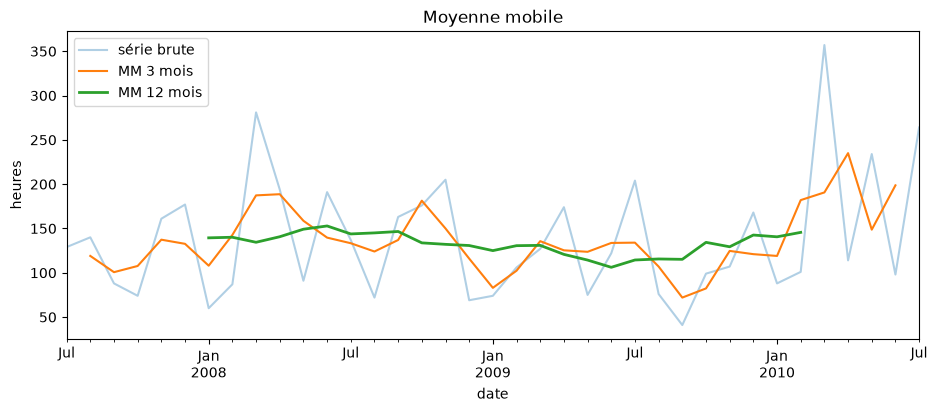
\includegraphics[width=\linewidth]{mm}
            \subcaption{Série brute et moyennes mobiles (3 et 12 mois).}
      \end{subfigure}\hfill
      \begin{subfigure}{0.42\linewidth}\centering
            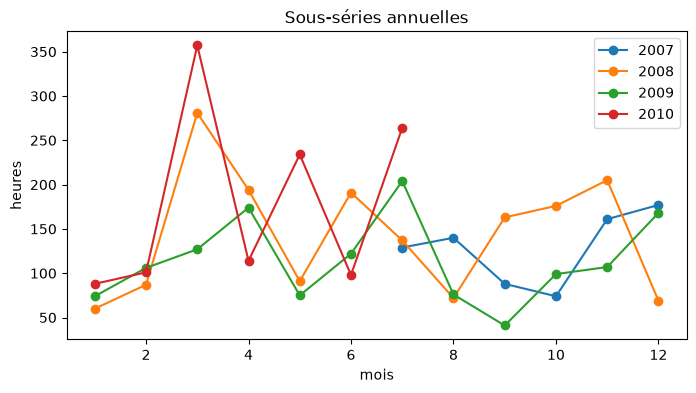
\includegraphics[width=\linewidth]{sousseries}
            \subcaption{Sous-séries annuelles superposées.}
      \end{subfigure}
      \caption{Tendance et profils annuels.}
      \label{fig:mm}
\end{figure}

\subsection{Décomposition saisonnière}

On décompose la série en \textbf{tendance $T$}, \textbf{saison $S$} et \textbf{résidu $R$}
selon trois approches (figures~\ref{fig:decomp}--\ref{fig:stl}) :
\begin{itemize}
      \item \textbf{Additif} $X = T + S + R$ : la saison s'ajoute en heures ;
      \item \textbf{Multiplicatif} $X = T \cdot S \cdot R$ : la saison est un facteur, utile
            quand l'amplitude croît avec le niveau ;
      \item \textbf{STL} (Loess, robuste aux points aberrants).
\end{itemize}

\begin{figure}[H]
      \centering
      \begin{subfigure}{0.49\linewidth}\centering
            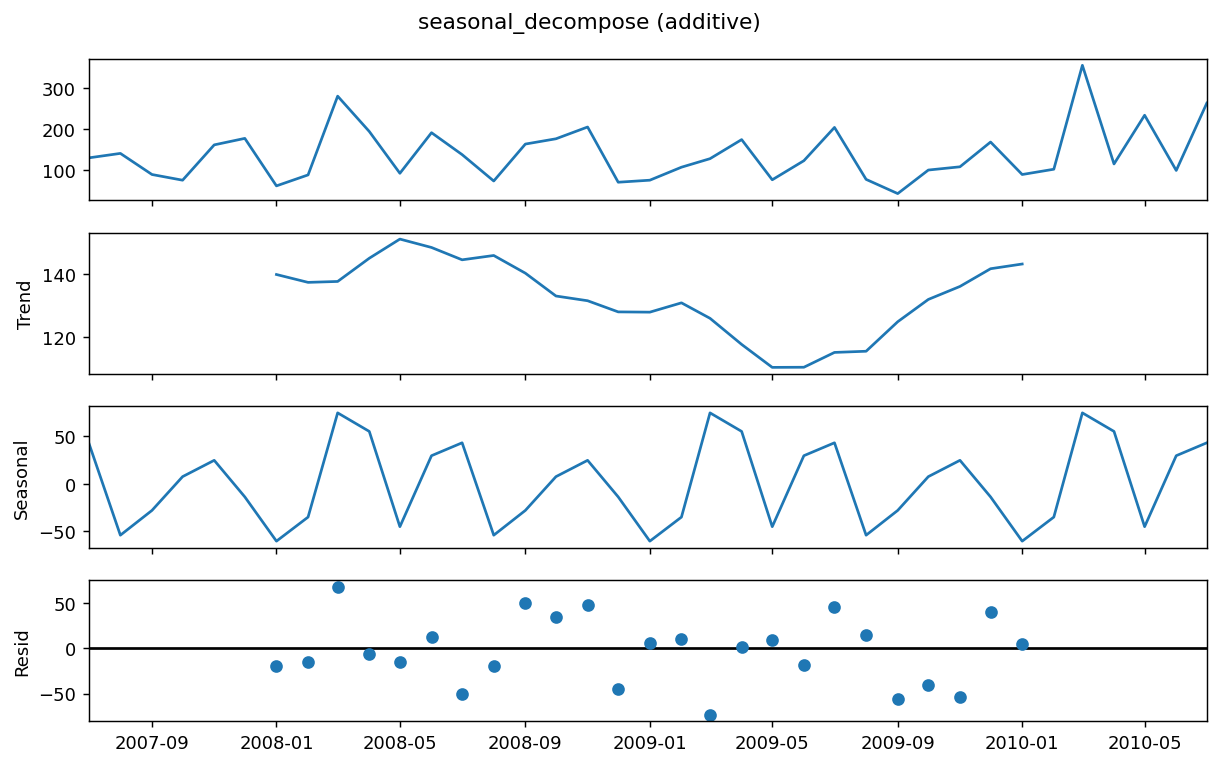
\includegraphics[width=\linewidth]{decomp}
            \subcaption{Additif ($X=T+S+R$)}
      \end{subfigure}\hfill
      \begin{subfigure}{0.49\linewidth}\centering
            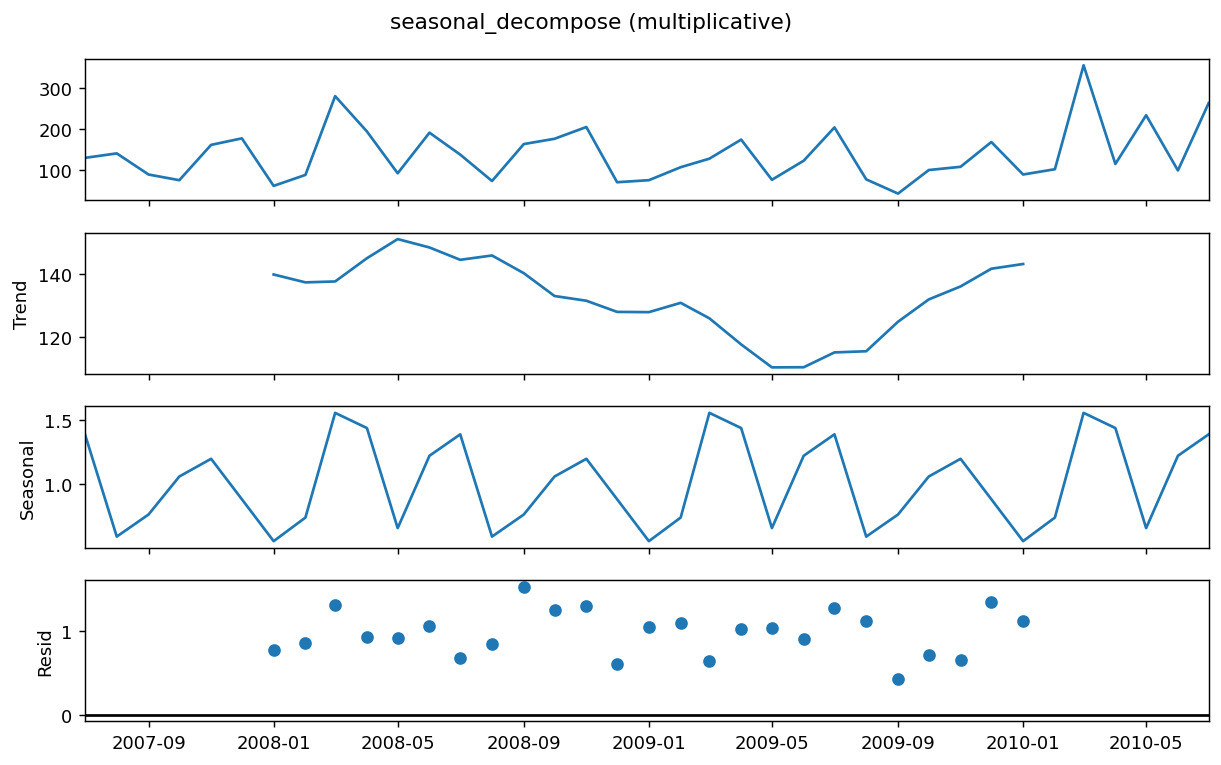
\includegraphics[width=\linewidth]{decomp1}
            \subcaption{Multiplicatif ($X=T\cdot S\cdot R$)}
      \end{subfigure}
      \caption{Décomposition par moyenne mobile.}
      \label{fig:decomp}
\end{figure}

\textbf{Lecture.} En \textbf{additif}, la saison a une amplitude de $\pm 50$ à $75$~h, du
\emph{même ordre} que les résidus ($\pm 50$--$70$~h) : la saison \alert{ne domine pas le
      bruit}. En \textbf{multiplicatif}, le facteur saisonnier oscille entre $\sim\!0{,}6$ et
$\sim\!1{,}55$ (certains mois nettement au-dessus du niveau local, d'autres en dessous),
même forme répétée : \emph{effet visible mais pas écrasant}.

\begin{figure}[H]
      \centering
      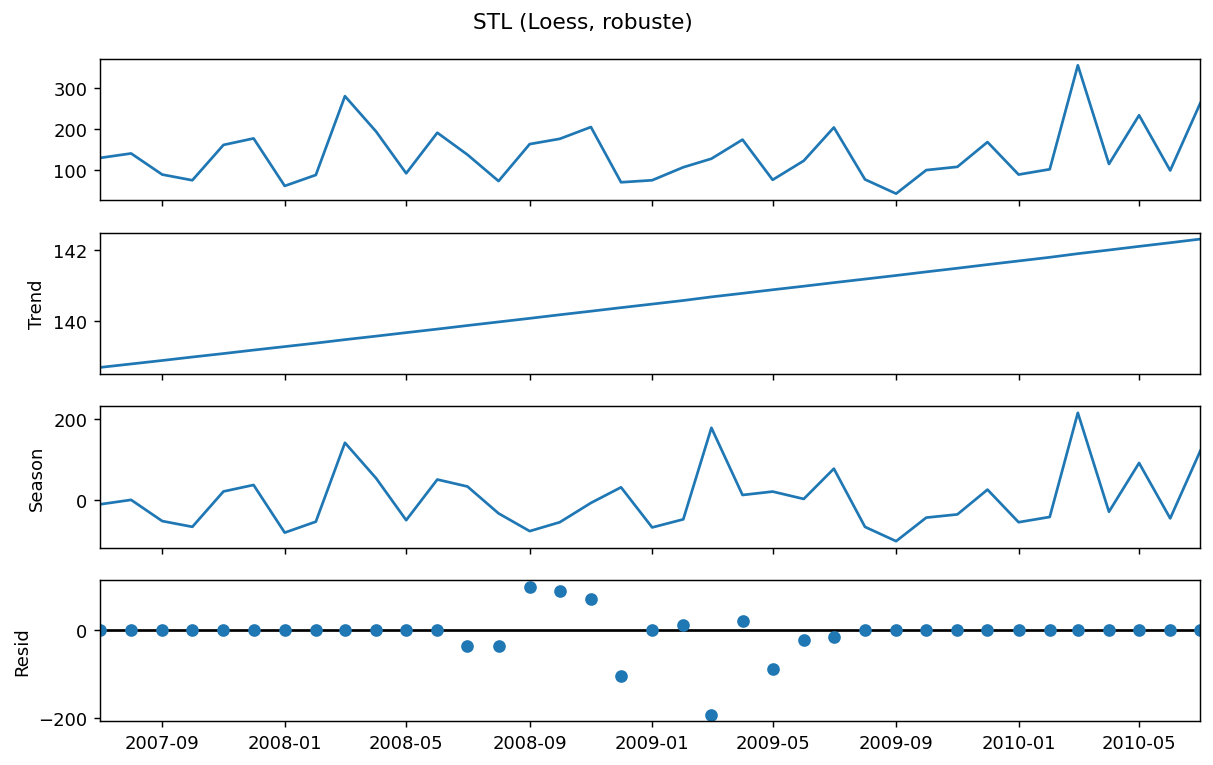
\includegraphics[width=0.72\linewidth]{decomp2}
      \caption{Décomposition \textbf{STL} (Loess, robuste). La tendance ressort en droite quasi
            linéaire.}
      \label{fig:stl}
\end{figure}

\textbf{Désaccord sur la tendance.} Additif et multiplicatif donnent une tendance
\emph{creuse} (en cuvette), alors que STL renvoie une \emph{droite} croissante : les deux
méthodes \alert{ne s'accordent pas} sur la tendance. On en conclut que le profil saisonnier
n'est \textbf{pas stable}. La cause principale est le manque de données : seulement
\textbf{3 cycles} de 12 mois, trop peu pour estimer une saison fiable. \emph{Conséquence
      directe : une modélisation \textbf{SARIMA} n'est pas justifiée a priori.}

\subsection{Stationnarité}

Avant de modéliser par ARMA/ARIMA, la série doit être \textbf{stationnaire} (moyenne,
variance et autocorrélation stables dans le temps). On combine une inspection visuelle
(moyenne et écart-type mobiles sur 12 mois, figure~\ref{fig:stat}) et deux tests aux
hypothèses \emph{opposées} :
\begin{itemize}
      \item \textbf{ADF} (H0 : racine unitaire, i.e. non stationnaire) : $p = 0{,}000$
            $\Rightarrow$ on rejette H0 ;
      \item \textbf{KPSS} (H0 : stationnaire) : $p = 0{,}100$ $\Rightarrow$ on ne rejette pas H0.
\end{itemize}
Les deux concordent : la série est \alert{stationnaire}, donc l'ordre d'intégration est
$\boxed{d = 0}$ — pas besoin de différencier, ce qui oriente directement vers un
$\text{ARIMA}(p,0,q)$.

\begin{figure}[H]
      \centering
      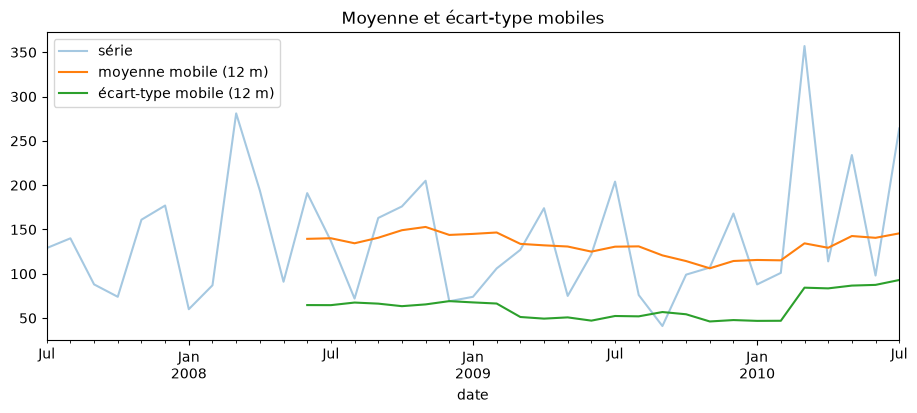
\includegraphics[width=0.82\linewidth]{stationnarite}
      \caption{Série, moyenne mobile et écart-type mobile (12 mois). Pas de tendance ni de
            gonflement de variance marqués.}
      \label{fig:stat}
\end{figure}

\subsection{Différenciation}

À titre de contrôle, on applique l'opérateur de différenciation
$\nabla = (1-B)$, soit $\nabla X_t = X_t - X_{t-1}$ (variation d'un mois à l'autre,
figure~\ref{fig:diff}). ADF et KPSS déclarent toujours la série stationnaire --- normal,
différencier une série déjà stationnaire le reste. Mais les tests ne suffisent pas : en
comparant l'\textbf{écart-type} et l'\textbf{ACF} avant/après, on constate que la
différenciation \alert{augmente} la variance et crée une forte autocorrélation négative au
lag~1 : c'est de la \textbf{sur-différenciation}. On garde donc $d = 0$.

\begin{figure}[H]
      \centering
      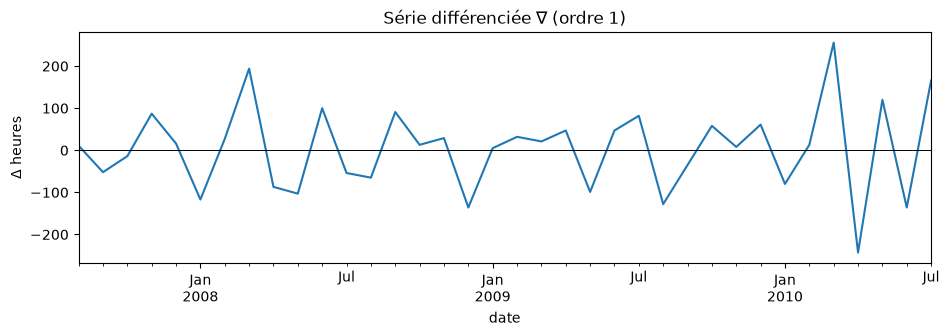
\includegraphics[width=0.78\linewidth]{diff}
      \caption{Série différenciée $\nabla$ (ordre 1) : oscillation autour de 0, signe de
            sur-différenciation.}
      \label{fig:diff}
\end{figure}
\newpage
\subsection{ACF / PACF}

Les corrélogrammes (figure~\ref{fig:acfpacf}) confirment le diagnostic :
\begin{itemize}
      \item \textbf{Série brute --- ACF} : décroissance immédiate (stationnaire) et
            \emph{aucun pic au lag~12} $\Rightarrow$ pas de saisonnalité annuelle exploitable.
      \item \textbf{Série brute --- PACF} : structure autorégressive faible, un petit ordre $p$
            suffit. ACF et PACF quasi plates $\Rightarrow$ série \alert{proche d'un bruit blanc}.
      \item \textbf{Série différenciée} : gros pic négatif au lag~1 ($\approx -0{,}47$) et
            spikes décroissants sur la PACF, signature d'une composante MA(1) \emph{induite} par
            la sur-différenciation.
\end{itemize}
La PACF servira à fixer l'ordre $p$ de l'AR, l'ACF l'ordre $q$ du MA.

\begin{figure}[H]
      \centering
      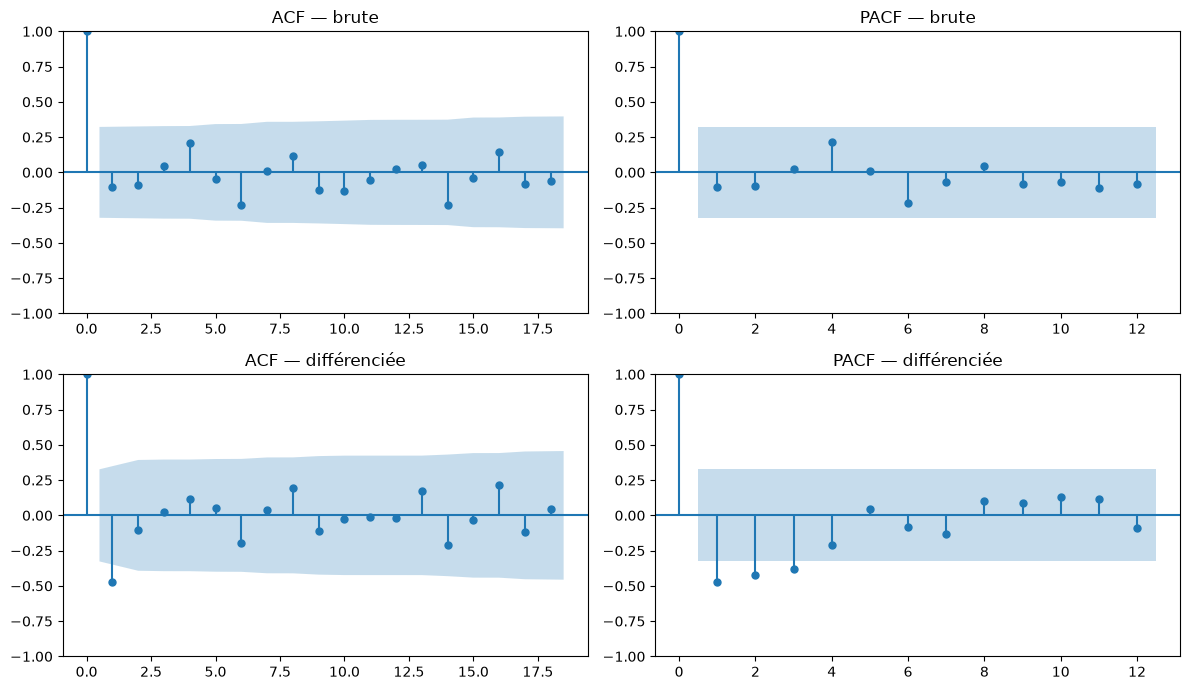
\includegraphics[width=\linewidth]{acfpacf}
      \caption{ACF et PACF de la série brute (haut) et différenciée (bas).}
      \label{fig:acfpacf}
\end{figure}
\newpage
\subsection{Mois de pic : quels motifs ?}

Le mois le plus chargé est \textbf{mars 2010}. En décomposant ce mois par motif
(figure~\ref{fig:pic}), le top en heures est \emph{ex æquo} :
\textbf{maladies de la peau} (112~h) et \textbf{traumatismes / causes externes} (112~h). Le
pic n'a donc \alert{pas de cause unique} : c'est un mélange d'accidents et de maladies.

\begin{figure}[H]
      \centering
      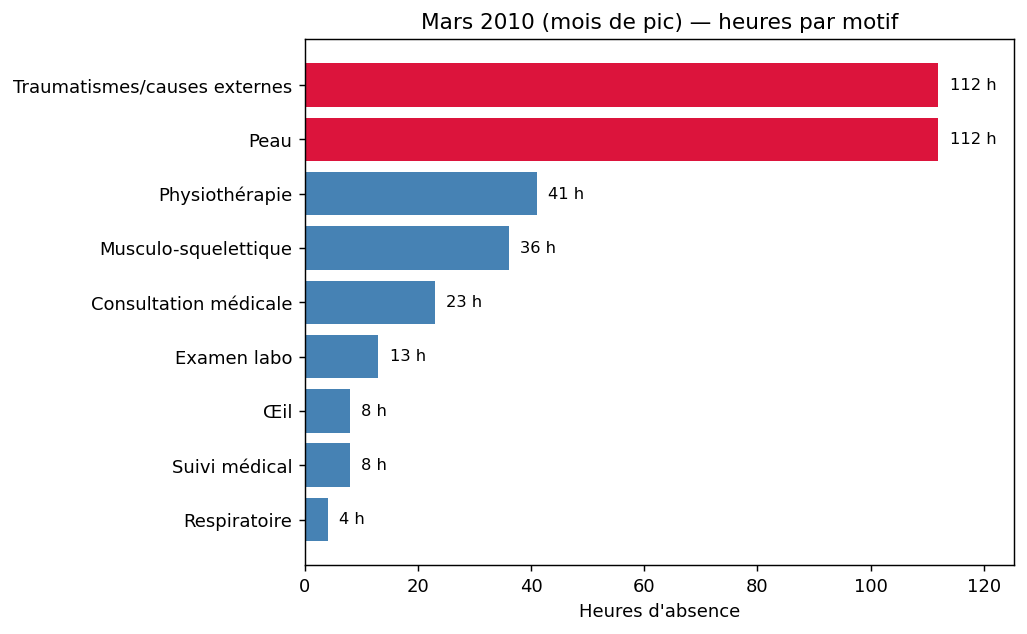
\includegraphics[width=0.72\linewidth]{pic_mars}
      \caption{Mars 2010 (mois de pic) : heures d'absence par motif. Les deux premiers postes
            sont à égalité (112~h).}
      \label{fig:pic}
\end{figure}

\textit{Hypothèse contextuelle (non prouvée).} Ce profil est compatible avec la
\textbf{saison des pluies} brésilienne du début 2010 (accidents et infections cutanées liés
aux intempéries), sur fond d'épidémie de dengue documentée dans l'État de São~Paulo. À
prendre avec prudence : l'année est \emph{reconstruite}.

%======================================================
\section{Prévision (forecasting)}

\subsection{Cadre \& baselines}

\textbf{Objectif :} anticiper le volume mensuel d'heures pour la planification RH. On
découpe la série en \textbf{train (28 mois)} / \textbf{test (9 mois)} de façon
chronologique. Deux modèles sont écartés d'emblée : \textbf{SARIMA} (pas de saison stable,
partie~2) et le ``I'' d'\textbf{ARIMA} (série déjà stationnaire, $d=0$, donc ARIMA $=$ ARMA).

On mesure l'erreur par \textbf{MAE} (erreur typique en heures, interprétable) et
\textbf{RMSE} (sanctionne les gros écarts, utile en RH pour éviter les grosses
sous-estimations ; sert au classement). Un modèle n'a de valeur que s'il bat la meilleure
\textbf{baseline} :

\begin{table}[H]
      \centering
      \begin{tabular}{lcc}
            \toprule
            Baseline                           & MAE  & RMSE         \\ \midrule
            \alert{moyenne} (moyenne du train) & 71,5 & \alert{98,5} \\
            naïf (dernière valeur)             & 73,8 & 114,1        \\
            naïf saisonnier (valeur à $t-12$)  & 83,2 & 108,3        \\ \bottomrule
      \end{tabular}
      \caption{Baselines sur le test. Référence à battre : \textbf{moyenne} (RMSE 98,5).}
\end{table}

\subsection{Modèles AR($p$), MA($q$) et ARMA($p,0,q$)}

\textbf{AR($p$) --- autorégression.} Applicable car la série est stationnaire ; l'ordre $p$
est le dernier lag significatif de la \textbf{PACF} ($-0{,}48$), d'où \textbf{AR(2)}, estimé
par MLE.

\textbf{MA($q$) --- moyenne mobile.} Même principe, l'ordre $q$ est le dernier lag
significatif de l'\textbf{ACF}, d'où \textbf{MA(2)}.

\textbf{ARMA($p,0,q$) --- Box-Jenkins.} On balaie la grille $(p,q)$ et on sélectionne par
critère d'information. On retient le \textbf{BIC} (min) car il pénalise plus la complexité
que l'AIC ($\ln T$ contre $2$ par paramètre), donc plus \emph{parcimonieux} et consistant.
Le BIC minimal désigne \textbf{ARMA(0,2) $=$ MA(2)}. \emph{Remarque :} AR et MA sont des cas
particuliers d'ARMA ; la grille confirme qu'aucun modèle \emph{mixte} ne fait mieux.

\begin{table}[H]
      \centering
      \begin{tabular}{lcc}
            \toprule
            Modèle              & MAE  & RMSE         \\ \midrule
            \alert{AR(2)}       & 70,6 & \alert{96,3} \\
            MA(2) $=$ ARMA(0,2) & 70,6 & 97,7         \\
            moyenne (baseline)  & 71,5 & 98,5         \\ \bottomrule
      \end{tabular}
      \caption{Comparaison sur le test. Le meilleur RMSE est obtenu par \textbf{AR(2)}.}
\end{table}

\textbf{Bilan chiffré.} Tous les modèles battent les baselines naïves, mais \emph{à peine} la
moyenne : 96,3 contre 98,5, soit $\sim\!2\,\%$ de mieux seulement. Autrement dit, prédire
``intelligemment'' ne fait guère mieux que prédire la moyenne — confirmation que la série est
\alert{proche d'un bruit blanc}, avec très peu de dynamique exploitable.

\subsection{Diagnostic des résidus (Box-Jenkins)}

Un modèle est validé si ce qu'il n'explique pas ressemble à un \textbf{bruit blanc}
(figure~\ref{fig:residus}). L'ACF des résidus est \textbf{plate} (toutes les barres dans la
bande de confiance, aucune autocorrélation significative) et les résidus oscillent autour de
0 sans motif. Le test de \textbf{Ljung-Box} (H0 : pas d'autocorrélation jusqu'au lag $k$)
confirme :

\begin{table}[H]
      \centering
      \begin{tabular}{ccc}
            \toprule
            lag $k$ & \texttt{lb\_stat} ($Q$) & \texttt{lb\_pvalue} \\ \midrule
            6       & 1,802                   & \alert{0,937}       \\
            12      & 6,744                   & \alert{0,874}       \\ \bottomrule
      \end{tabular}
      \caption{Ljung-Box sur les résidus. $p \gg 0{,}05$ aux deux horizons (court terme et cycle
            annuel) $\Rightarrow$ on ne rejette pas H0.}
\end{table}

Les résidus sont donc \alert{compatibles avec un bruit blanc}. (À noter : Ljung-Box teste
l'autocorrélation, \emph{pas} la normalité.)

\begin{figure}[H]
      \centering
      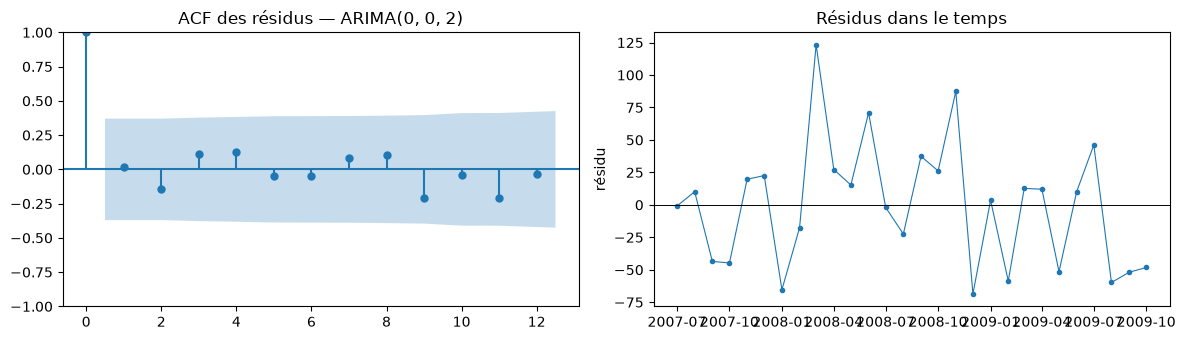
\includegraphics[width=0.9\linewidth]{residus}
      \caption{ACF des résidus (gauche) et résidus dans le temps (droite) pour le modèle retenu.}
      \label{fig:residus}
\end{figure}

\subsection{Résultats \& projection}

La figure~\ref{fig:prev} montre la prévision sur le jeu de test (avec IC~95\,\%) puis la
projection des 12 mois suivants. On ne reproduit clairement pas la dynamique : même avec le
meilleur modèle, la série reste très proche d'un bruit blanc, sans saisonnalité ni
corrélation exploitable.

\begin{figure}[H]
      \centering
      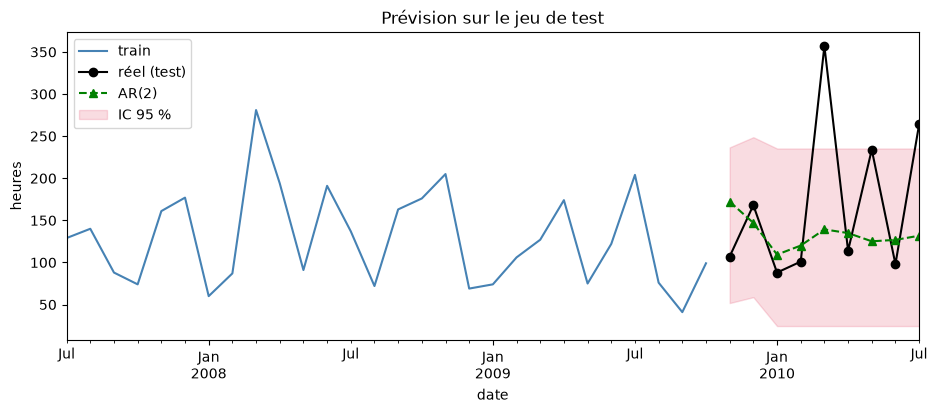
\includegraphics[width=0.85\linewidth]{prev_test}
      \caption{Prévision sur le test (AR(2) et ARMA) avec intervalle de confiance à 95\,\%.}
      \label{fig:prev}
\end{figure}

\paragraph{Conclusion (prévision).} Les modèles ne battent guère la moyenne et les résidus
sont déjà un bruit blanc : la série mensuelle porte \alert{peu de dynamique exploitable}.
D'où le \textbf{pivot} vers une approche explicative.

\paragraph{Pistes d'amélioration (prévision).}
\begin{itemize}
  \item \textbf{Granularité plus fine} : travailler en données hebdomadaires/journalières
        plutôt que mensuelles (37 points sont trop peu) pour capter une dynamique.
  \item \textbf{Variables exogènes} (SARIMAX) : intégrer charge de travail, jours fériés,
        saison comme régresseurs externes plutôt que la seule série.
  \item \textbf{Modèles non linéaires} (lissage exponentiel, gradient boosting sur features
        calendaires) une fois davantage d'historique disponible.
\end{itemize}

%======================================================
\section{Approche explicative --- effet du jour de la semaine}

Le forecasting mensuel n'ayant rien donné, on analyse l'effet du \textbf{jour de la semaine}
(lundi → vendredi, sans week-end), seule dimension temporelle fine fiable. Il s'agit d'une
analyse \emph{descriptive + tests}, pas d'une prévision.

\textbf{Durée selon le jour.} Le \emph{nombre} d'absences est homogène selon le jour
(125--161), mais c'est la \emph{durée moyenne} qui varie : élevée le \textbf{lundi}
(9,2~h, bien au-dessus de la moyenne globale $\sim\!6{,}9$~h), décroissante jusqu'au jeudi
(4,4~h), léger rebond le vendredi (5,2~h) --- figure~\ref{fig:jour}. Un test de
\textbf{Kruskal-Wallis} (comparaison non paramétrique des distributions entre les 5 groupes)
donne $H = 10{,}7$, $p = 0{,}030 < 0{,}05$ : on rejette H0, \alert{au moins un jour diffère}.

\begin{figure}[H]
      \centering
      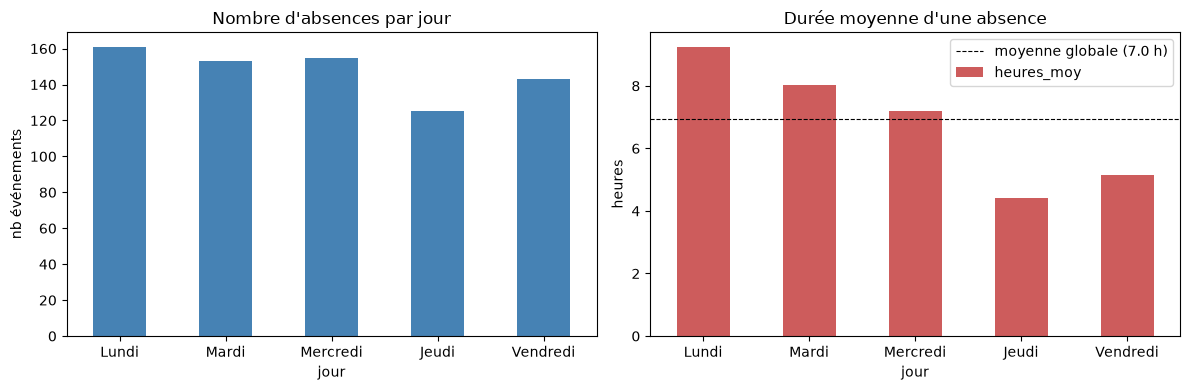
\includegraphics[width=0.9\linewidth]{jour}
      \caption{Nombre d'absences (gauche) et durée moyenne (droite) par jour de la semaine.}
      \label{fig:jour}
\end{figure}

\textbf{Risque d'absence longue.} On définit une cible binaire : absence \textbf{longue}
$= $ plus de 8~h (au-delà d'une journée standard). Le taux d'absence longue varie selon le
jour (figure~\ref{fig:jourlong}). Un test du \textbf{$\chi^2$ d'indépendance} (H0 : le jour
et ``absence longue'' sont indépendants) donne $p = 0{,}021 < 0{,}05$ : on rejette H0, le
risque d'absence longue \alert{dépend du jour}.

\begin{figure}[H]
      \centering
      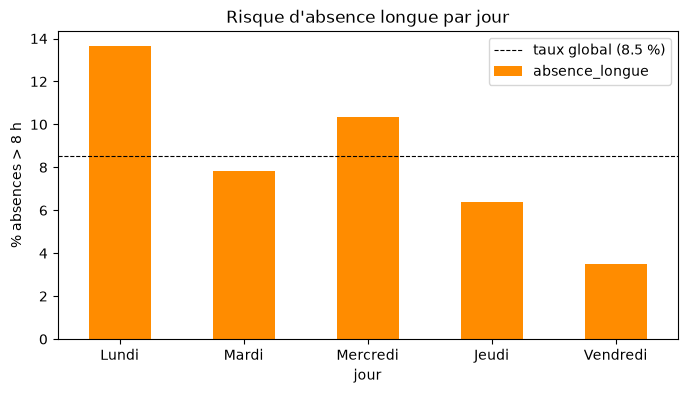
\includegraphics[width=0.62\linewidth]{jour_long}
      \caption{Taux d'absences $>8$~h par jour, comparé au taux global.}
      \label{fig:jourlong}
\end{figure}

\textbf{Conclusion.} Le jour de la semaine est un prédicteur \alert{pertinent et cohérent},
que l'on conserve comme variable pour la classification.

%======================================================
\section{Classification de la durée d'absence}

\textbf{Problématique.} Classer une absence en trois classes de durée :
\textbf{low} ($\leq 4$~h), \textbf{mod} (5--8~h) ou \textbf{high} ($>8$~h). Les classes sont
\alert{déséquilibrées} (458 / 216 / 63, soit $\approx 62\,/\,29\,/\,8{,}5\,\%$), ce qui écarte
l'\emph{accuracy} : on évalue par \textbf{macro-F1}, \textbf{balanced accuracy} et
\textbf{ROC-AUC (ovr)}, qui traitent les trois classes à égalité.

\textbf{Protocole.} Pipeline \texttt{préprocessing → modèle} (one-hot pour les
catégorielles, standardisation pour les numériques), split \textbf{stratifié 75/25} +
\textbf{validation croisée 5-fold}, avec repondération des classes. Cinq modèles sont
comparés.

\subsection{Séparabilité des classes}

Une projection \textbf{PCA 2D} des données prétraitées (figure~\ref{fig:pca}) montre un
\alert{fort chevauchement} des trois classes (pas de clusters nets, $\sim\!34\,\%$ de
variance capturée en 2D). La difficulté de classification vient donc \emph{des données
      elles-mêmes}.

\begin{figure}[H]
      \centering
      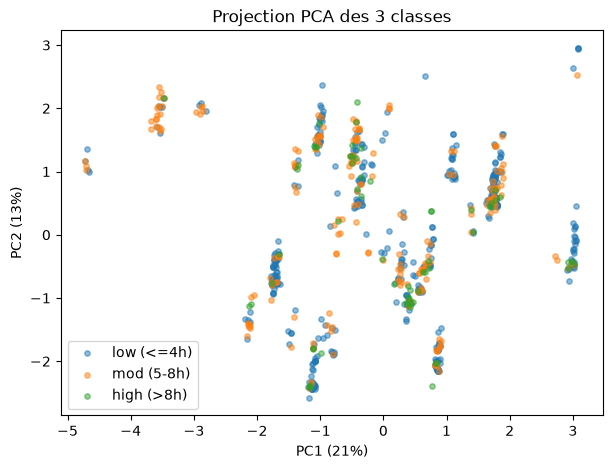
\includegraphics[width=0.62\linewidth]{pca}
      \caption{Projection PCA 2D colorée par classe : les classes se recouvrent largement.}
      \label{fig:pca}
\end{figure}

\subsection{Comparaison des modèles}

\begin{table}[H]
      \centering
      \begin{tabular}{lcccc}
            \toprule
            Modèle                        & CV F1-macro   & test F1-macro & ROC-AUC (ovr) & bal-acc \\ \midrule
            Baseline (majoritaire)        & 0,256         & 0,256         & 0,500         & 0,333   \\
            \alert{Régression logistique} & \alert{0,611} & 0,592         & 0,823         & 0,636   \\
            Arbre de décision             & 0,518         & 0,467         & 0,639         & 0,470   \\
            SVM                           & 0,576         & 0,560         & \alert{0,842} & 0,586   \\
            Random Forest                 & 0,595         & 0,581         & 0,838         & 0,584   \\ \bottomrule
      \end{tabular}
      \caption{Performances (validation croisée et test). Meilleur macro-F1 : régression
            logistique ; meilleur ROC-AUC : SVM.}
\end{table}

Tous les modèles \alert{écrasent la baseline} (0,26). Le meilleur en \textbf{macro-F1} est la
\textbf{régression logistique} (CV 0,61), devant Random Forest (0,59) et SVM (0,58) ; l'arbre
seul est le plus faible (0,52). SVM et RF dominent en \textbf{ROC-AUC ovr} ($\sim\!0{,}84$).
Fait notable : un modèle \textbf{simple} (régression logistique) rivalise avec le Random
Forest.

\subsection{Analyse par classe}

La matrice de confusion et le rapport par classe (figure~\ref{fig:conf}) précisent où ça
coince :
\begin{itemize}
      \item \textbf{low} ($\leq 4$~h) : bien classée, \textbf{F1 $\approx 0{,}85$} (classe
            majoritaire, features nettes) ;
      \item \textbf{mod} (5--8~h) : \textbf{F1 $\approx 0{,}57$}, classe \emph{ambiguë} coincée
            entre les deux autres (frontières floues) ;
      \item \textbf{high} ($>8$~h) : \textbf{rappel $0{,}56$} mais \textbf{précision $0{,}26$}
            (F1 $\approx 0{,}35$) --- rare (63 obs), le modèle ratisse large et multiplie les
            faux positifs.
\end{itemize}
$\Rightarrow$ une \alert{difficulté intrinsèque aux données} (déséquilibre + chevauchement),
que confirme la PCA.

\begin{figure}[H]
      \centering
      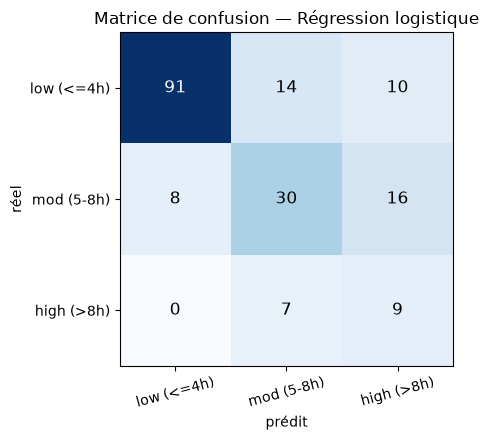
\includegraphics[width=0.6\linewidth]{confusion}
      \caption{Matrice de confusion du meilleur modèle (au sens macro-F1).}
      \label{fig:conf}
\end{figure}

\paragraph{Pistes d'amélioration (classification).}
\begin{itemize}
  \item \textbf{Rééquilibrage} de la classe rare \emph{high} : sur-échantillonnage
        \textbf{SMOTE} ou ajustement du \textbf{seuil} de décision (au lieu de $0{,}5$) pour
        remonter la précision.
  \item \textbf{Modèles plus expressifs} : \textbf{gradient boosting} (XGBoost / LightGBM),
        avec réglage d'hyperparamètres.
  \item \textbf{Feature engineering} : exploiter l'\textbf{historique par employé} (via
        \texttt{ID}) --- nombre d'absences passées, durée moyenne individuelle.
\end{itemize}

\subsection{Variables les plus discriminantes}

Les importances du Random Forest (figure~\ref{fig:imp}) placent en tête la \textbf{charge de
      travail} ($\sim\!9\,\%$), l'\textbf{atteinte d'objectif} (\emph{Hit target}, $\sim\!7{,}6\,\%$)
puis le \textbf{motif}. Le \textbf{jour de la semaine} pèse $\sim\!10\,\%$ cumulé, ce qui
\alert{confirme} l'effet établi en partie~4.

\begin{figure}[H]
      \centering
      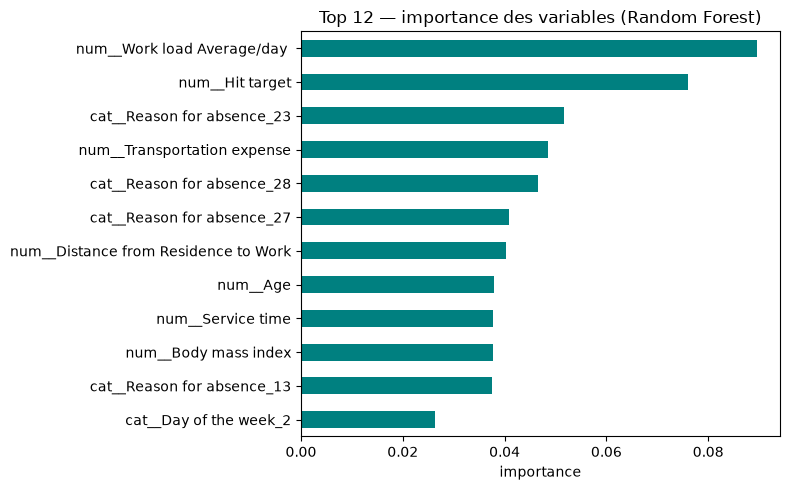
\includegraphics[width=0.62\linewidth]{importances}
      \caption{Top 12 des variables par importance (Random Forest).}
      \label{fig:imp}
\end{figure}

%======================================================
\clearpage
\section{Conclusion générale}

\textbf{Prévision.} La série mensuelle est courte (37 points), stationnaire ($d=0$), sans
saisonnalité stable (SARIMA écarté) et \alert{proche d'un bruit blanc} : les modèles
AR/MA/ARMA ne dépassent la moyenne que de $\sim\!2\,\%$ et les résidus sont déjà un bruit
blanc. Il y a donc \emph{peu de dynamique à exploiter}.

\textbf{Explication.} Le pivot vers l'analyse descriptive est plus fructueux : le
\textbf{jour de la semaine} influe significativement sur la durée (Kruskal-Wallis) et sur le
risque d'absence longue ($\chi^2$). En classification, les absences courtes sont bien
prédites, mais la classe \textbf{high} reste dure (rare et chevauchante) : la limite vient
\alert{des données}, pas des modèles.

\textbf{Recontextualisation \& perspectives.} Pour un usage RH réel, la valeur n'est donc pas
dans la prévision du volume mensuel mais dans l'\textbf{explication} : le jour de
la semaine est un levier actionnable . Pour aller plus loin, il faudrait
\alert{enrichir les données} :
\begin{itemize}
  \item collecter un \textbf{historique plus long et plus fin} (hebdomadaire) et des
        \textbf{variables exogènes} (jours fériés, charge) pour rendre la prévision utile ;
  \item suivre les absences \textbf{par employé} (\texttt{ID}) pour passer d'une vue agrégée à
        un modèle individuel du risque d'absence ;
\end{itemize}

\end{document}
